\documentclass[11pt, oneside]{article}   	% use "amsart" instead of "article" for AMSLaTeX format
\usepackage[top=1.3in,bottom=1in,right=1in,left=1in,headheight=30pt]{geometry}

\geometry{letterpaper}                   		% ... or a4paper or a5paper or ...
%\geometry{landscape}                		% Activate for rotated page geometry
%\usepackage[parfill]{parskip}    		% Activate to begin paragraphs with an empty line rather than an indent
\usepackage{graphicx}				% Use pdf, png, jpg, or eps§ with pdflatex; use eps in DVI mode
\usepackage{pdfpages}
\usepackage{pgfplots, xcolor}
\usepackage{amsmath,amsthm,amssymb,amsfonts} 	%Prooflandia
\usepackage[utf8]{inputenc}
\usepackage{amssymb}
\makeatother
\usepackage{pifont}
\usepackage{marvosym, wasysym, graphicx, wrapfig, placeins, subcaption, booktabs}
 \usepackage{cancel, framed, topcapt}
 \usepackage{tikz, pgfplots, pifont}
 \usepackage [autostyle, english = american]{csquotes}
	\MakeOuterQuote{"}
\usepackage{fancyhdr}
\pagestyle{fancy}
\lhead{Modeling Complex Systems --- CSYS/CS 302\\
Assignment 02  \\
Date: \today
} %%%%%%%%%%%% PUT IN ASSIGNMENT # %%%%%%%%%%%%
\rhead{Sarah Howerter\\
Daniel Berenberg}
\cfoot{\thepage}

\usepackage[colorlinks=true, pdfstartview=FitV, linkcolor=blue,
            citecolor=blue, urlcolor=blue]{hyperref}
            \usepackage{color}
            \definecolor{dkgreen}{rgb}{0,0.6,0}
            \definecolor{gray}{rgb}{0.5,0.5,0.5}
            \definecolor{mauve}{rgb}{0.58,0,0.82}
            \usepackage{listings}
            \lstset{frame=tb,
              language=python,
              aboveskip=3mm,
              belowskip=3mm,
              showstringspaces=false,
              columns=flexible,
              basicstyle={\footnotesize\ttfamily},
              numbers=none,
              numberstyle=\tiny\color{gray},
              keywordstyle=\color{blue},
              commentstyle=\color{dkgreen},
              stringstyle=\color{mauve},
              breaklines=true,
              breakatwhitespace=true,
              tabsize=3
            }

\newcommand{\N}{\mathbb{N}}
\newcommand{\Z}{\mathbb{Z}}
\newcommand{\bt}{$\bullet$}
\newcommand{\cmdin}{$>$}
\newcommand{\cmdout}{[1]}
%SetFonts
%\, = insert small space
%\textrm{} = sets to text form inside math land
%SetFonts

\newcommand{\prob}[2]{
\indent \\
\noindent{\color{green!50!blue}\bf {\large#1.}}
{\normalfont #2}
}
\newcommand{\Prob}{\textrm{{\bf Pr}}}

\begin{document}
\prob{1}{See code. Filenames:}\\
	\indent Driver script: \texttt{L\_system.py} \\
	\indent L-system expansion script: \texttt{L\_sysExpand.py} \\
	\indent L-system plotting script: \texttt{L\_sysDraw.py}\\
	This \texttt{L\_system.py} python script can be run by anyone and asks the user (in the command line) to either choose which L-system they would like to create (tree or snowflake) or gives them the option to input their own axiom and rules. It also gives the options to set up the drawing parameters of the system and whether or not to randomize the ``turtle'' step lengths and turning angles.

\prob{2}{We decided to recreate the L-system for the tree example that is on the explorables website and incorporate the randomization of branch lenghts and angles. We also wanted to create an L-system for a snowflake and used the following setup:\\
	\indent $\bullet$ {\bf axiom:}
	[G]+[G]+[G]+[G]+[G]+[G]
	\\
	\indent $\bullet$ {\bf rules:}}
	G $\rightarrow$ `F[-G][GG][+G]' and F $\rightarrow$ `FF'
	\begin{figure}[h!]
		\centering
		\vspace{-3mm}
		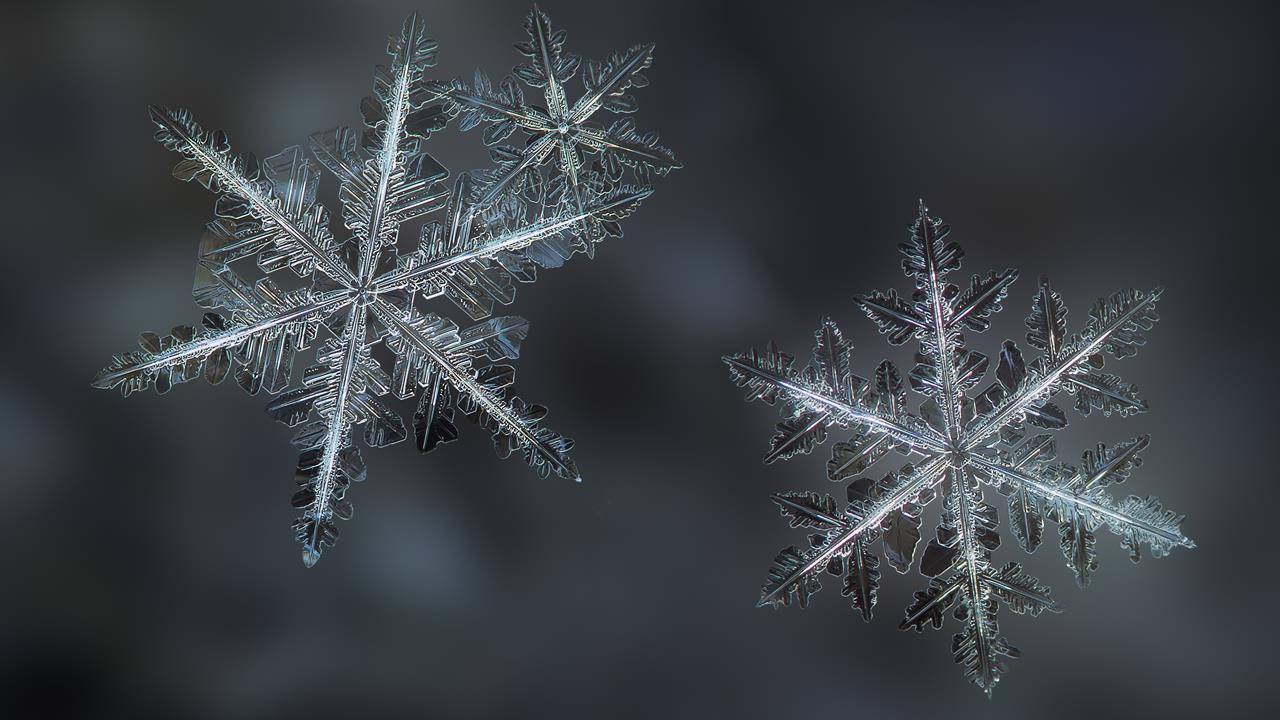
\includegraphics[width=0.7\textwidth]{figs/snowflake}
		\begin{tabular}{lll}
			\includegraphics[width=0.36\textwidth]{figs/L-system_plots/L-sys--snowflake-007.pdf}
			&			\hspace{-9mm}
			\includegraphics[width=0.36\textwidth]{figs/L-system_plots/L-sys--snowflake-008.pdf}
			&			\hspace{-9mm}
			\includegraphics[width=0.36\textwidth]{figs/L-system_plots/L-sys--snowflake-009.pdf}
		\end{tabular}
		\vspace{-12mm}\caption{Snowflake image in nature \& Snowflake L-system drawings with 4, 5, and 6 iterations.}
		\label{snowflake_plots}
	\end{figure}

	\hspace{-2mm}\begin{figure}[h!]
		\centering
		\vspace{-3mm}
		\hspace{-6mm}\begin{tabular}{lll}
			\includegraphics[width=0.36\textwidth]{figs/L-system_plots/L-sys--tree-001.pdf}
			&			\hspace{-9mm}
			\includegraphics[width=0.36\textwidth]{figs/L-system_plots/L-sys--tree-002.pdf}
			&			\hspace{-9mm}
			\includegraphics[width=0.36\textwidth]{figs/L-system_plots/L-sys--tree-003.pdf}
			\\
			\includegraphics[width=0.36\textwidth]{figs/L-system_plots/L-sys--tree-004.pdf}
			&			\hspace{-9mm}
			\includegraphics[width=0.36\textwidth]{figs/L-system_plots/L-sys--tree-005.pdf}
			&			\hspace{-9mm}
			\includegraphics[width=0.36\textwidth]{figs/L-system_plots/L-sys--tree-006.pdf}
		\end{tabular}
		\vspace{-3mm}\caption{Tree L-system drawings with 4, 5, and 6 iterations and with and without randomization of line lengths and angles.}
		\label{tree_plots}
	\end{figure}





\end{document}
